\section{Typeset Text}

Prepare your submissions on a word processor or typesetter.  Please
note that page layout may change slightly depending upon the printer
you have specified.  \LaTeX\ sometimes will create overfull lines
that extend into columns.  To attempt to combat this, the .cls
file has a command, {\textbackslash}sloppy, that essentially asks
\LaTeX\ to prefer underfull lines with extra whitespace.  For more
details on this, and info on how to control it more finely, check out
{\url{http://www.economics.utoronto.ca/osborne/latex/PMAKEUP.HTM}}.

\subsection{Title and Authors}

Your paper's title, authors and affiliations should run across the
full width of the page in a single column 17.8 cm (7 in.) wide.  The
title should be in Helvetica 18-point bold; use Arial if Helvetica is
not available.  Authors' names should be in Times Roman 12-point bold,
and affiliations in Times Roman 12-point.  For more than three authors,
you may have to place some address information in a footnote, or in a named
section at the end of your paper. Please use full international addresses and
telephone dialing prefixes.  Leave one 10-pt line of white space below the last
line of affiliations.

\subsection{Abstract and Keywords}

Every submission should begin with an abstract of about 150 words,
followed by a set of keywords. The abstract and keywords should be
placed in the left column of the first page under the left half of the
title. The abstract should be a concise statement of the problem,
approach and conclusions of the work described.  It should clearly
state the paper's contribution to the field of HCI.

The first set of keywords will be used to index the paper in the
proceedings. The second set are used to catalogue the paper in the ACM
Digital Library. The latter are entries from the ACM Classification
System~\cite{acm_categories}.  In general, it should only be necessary
to pick one or more of the H5 subcategories, see
\url{http://www.acm.org/class/1998/ccs98.html}

\subsection{Normal or Body Text}

Please use a 10-point Times Roman font or, if this is unavailable,
another proportional font with serifs, as close as possible in
appearance to Times Roman 10-point. The Press 10-point font available
to users of Script is a good substitute for Times Roman. If Times
Roman is not available, try the font named Computer Modern Roman. On a
Macintosh, use the font named Times and not Times New Roman. Please
use sans-serif or non-proportional fonts only for special purposes,
such as headings or source code text.

\subsection{First Page Copyright Notice}

Leave 3 cm (1.25 in.) of blank space for the copyright notice at the
bottom of the left column of the first page. In this template a
floating text box will automatically generate the required space. Note
however that the text box is anchored to the \textbf{ABSTRACT}
heading, so if that heading is deleted the text box will disappear as
well.  You can replace the default copyright notice by uncommenting
the {\textbackslash}toappear block at the beginning of the document
and inserting your own text, for example, for versions under review.


\subsection{Subsequent Pages}

On pages beyond the first, start at the top of the page and continue
in double-column format.  The two columns on the last page should be
of equal length.

\begin{figure}[!h]
\centering
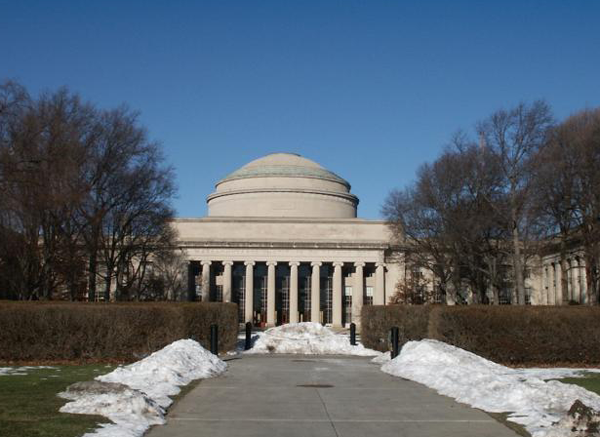
\includegraphics[width=0.9\columnwidth]{Figure1}
\caption{With Caption Below, be sure to have a good resolution image
  (see item D within the preparation instructions).}
\label{fig:figure1}
\end{figure}

\subsection{References and Citations}

Use a numbered list of references at the end of the article, ordered
alphabetically by first author, and referenced by numbers in brackets
\cite{ethics,
  Klemmer:2002:WSC:503376.503378,
  Mather:2000:MUT,
  Zellweger:2001:FAO:504216.504224}. For
papers from conference proceedings, include the title of the paper and
an abbreviated name of the conference (e.g., for Interact 2003
proceedings, use \textit{Proc. Interact 2003}). Do not include the
location of the conference or the exact date; do include the page
numbers if available. See the examples of citations at the end of this
document. Within this template file, use the \texttt{References} style
for the text of your citation.

Your references should be published materials accessible to the
public.  Internal technical reports may be cited only if they are
easily accessible (i.e., you provide the address for obtaining the
report within your citation) and may be obtained by any reader for a
nominal fee.  Proprietary information may not be cited. Private
communications should be acknowledged in the main text, not referenced
(e.g., ``[Robertson, personal communication]'').

\begin{table}
  \centering
  \begin{tabular}{|c|c|c|}
    \hline
    \tabhead{Objects} &
    \multicolumn{1}{|p{0.3\columnwidth}|}{\centering\tabhead{Caption --- pre-2002}} &
    \multicolumn{1}{|p{0.4\columnwidth}|}{\centering\tabhead{Caption --- 2003 and afterwards}} \\
    \hline
    Tables & Above & Below \\
    \hline
    Figures & Below & Below \\
    \hline
  \end{tabular}
  \caption{Table captions should be placed below the table.}
  \label{tab:table1}
\end{table}